\documentclass[10pt,a4paper]{article}

% --- PAQUETES BÁSICOS ---
\usepackage[utf8]{inputenc}
\usepackage[spanish,es-tabla]{babel}
\usepackage[top=2cm,bottom=2.2cm,left=2cm,right=2cm]{geometry}
\usepackage{amsmath,amssymb}
\usepackage{xcolor}
\usepackage{listings}
\usepackage{booktabs}
\usepackage{array}
\usepackage{tabularx}
\usepackage{fancyhdr}
\usepackage{graphicx}
\usepackage[hidelinks]{hyperref}
\usepackage{tcolorbox}
\tcbuselibrary{skins,breakable}
\usepackage{enumitem}

% --- CONFIGURACIÓN DE COLORES INSTITUCIONALES ---
\definecolor{unsaacblue}{RGB}{13, 71, 161}
\definecolor{accentblue}{RGB}{26, 115, 232}
\definecolor{darkgray}{RGB}{40, 40, 40}
\definecolor{lightgray}{RGB}{245, 247, 250}
\definecolor{codebg}{RGB}{248, 249, 251}
\definecolor{openstate}{RGB}{19, 115, 51}
\definecolor{closedstate}{RGB}{197, 34, 31}
\definecolor{filteredstate}{RGB}{176, 96, 0}

\newcommand{\TCP}{\textbf{TCP}}
\newcommand{\UDP}{\textbf{UDP}}

% --- CONFIGURACIÓN DE ENCABEZADO Y PIE DE PÁGINA ---
\pagestyle{fancy}
\fancyhf{}
\renewcommand{\headrulewidth}{0.6pt}
\renewcommand{\footrulewidth}{0.4pt}
\fancyhead[L]{\small\textbf{\color{unsaacblue}UNSAAC -- Dpto. Académico de Ingeniería Informática}}
\fancyhead[R]{\small\color{darkgray}Redes de Computadoras 2 | Lab 04}
\fancyfoot[L]{\small\color{darkgray}Estudiante: \textbf{Noe Franklin Choquenaira Quispe (Cód. 133962)}}
\fancyfoot[R]{\small\thepage}

% --- CONFIGURACIÓN DE LISTINGS (CÓDIGO FUENTE) ---
\lstset{
    language=Python,
    backgroundcolor=\color{codebg},
    basicstyle=\ttfamily\scriptsize\color{darkgray},
    keywordstyle=\bfseries\color{unsaacblue},
    stringstyle=\color{closedstate},
    commentstyle=\itshape\color{openstate},
    numberstyle=\tiny\color{gray},
    numbers=left,
    stepnumber=1,
    numbersep=6pt,
    tabsize=4,
    showspaces=false,
    showstringspaces=false,
    breaklines=true,
    breakatwhitespace=true,
    frame=single,
    rulecolor=\color{lightgray},
    xleftmargin=10pt,
    framexleftmargin=8pt,
    captionpos=b
}

\begin{document}

% ==========================================================
% ENCABEZADO FORMAL DEL INFORME
% ==========================================================
\begin{tcolorbox}[colback=lightgray,colframe=unsaacblue,arc=3mm,boxrule=1.2pt]
\begin{center}
    {\large\textbf{\color{unsaacblue}UNIVERSIDAD NACIONAL DE SAN ANTONIO ABAD DEL CUSCO}}\\[1mm]
    {\normalsize\textbf{FACULTAD DE INGENIERÍA ELÉCTRICA, ELECTRÓNICA, INFORMÁTICA Y MECÁNICA}}\\[0.5mm]
    {\small\textbf{DEPARTAMENTO ACADÉMICO DE INGENIERÍA INFORMÁTICA}}\\[2mm]
    {\Large\textbf{\color{unsaacblue}INFORME DE LABORATORIO N° 04}}\\[1.5mm]
    {\large\textbf{Lab04: Tarea Scanner de Puertos TCP, UDP}}\\[2mm]
    \rule{0.9\textwidth}{0.6pt}\\[2mm]
    \begin{tabularx}{0.95\textwidth}{Xr}
        \textbf{Asignatura:} Redes de Computadoras 2 & \textbf{Docente:} Manuel Aurelio Peñaloza Figueroa \\
        \textbf{Estudiante:} Noe Franklin Choquenaira Quispe & \textbf{Código de Estudiante:} 133962 \\
        
    \end{tabularx}
\end{center}
\end{tcolorbox}

\vspace{1mm}

% ==========================================================
% 1. INTRODUCCIÓN Y REQUERIMIENTOS DEL LABORATORIO
% ==========================================================
\section{Introducción y Requerimientos del Laboratorio}

El escaneo de puertos permite examinar un host para identificar servicios de red en ejecución y posibles vulnerabilidades de seguridad. El presente trabajo detalla el desarrollo de una aplicación integral con \textbf{Interfaz Gráfica de Usuario (GUI)} en Python, capaz de escanear puertos en los protocolos \TCP{} y \UDP{}, desarrollada de manera autónoma cumpliendo estrictamente con los requerimientos técnicos de la guía de práctica del curso.

\subsection{Matriz de Requerimientos Funcionales}
\begin{table}[h!]
\centering\small
\begin{tabularx}{\textwidth}{lXl}
\toprule
\textbf{Requerimiento} & \textbf{Descripción Técnica de la Solución} & \textbf{Estado} \\
\midrule
Host dinámico & Entrada que acepta direcciones IPv4 (\texttt{127.0.0.1}) y nombres de dominio FQDN (\texttt{unsaac.edu.pe}). & Cumplido \\
Rango de puertos & Selección dinámica de puerto inicial y final con validación de límites (1 a 65535). & Cumplido \\
Selector de protocolo & RadioButtons interactivos para seleccionar independientemente: \TCP{}, \UDP{} o Ambos. & Cumplido \\
Interfaz Gráfica (GUI) & Diseñada con Tkinter y ttk, visualizando en tiempo real cada puerto con códigos de color. & Cumplido \\
No congelamiento & Ejecución concurrente multihilo (\texttt{ThreadPoolExecutor}) sin bloquear el hilo principal. & Cumplido \\
Exportación & Botón de guardado de resultados a archivos de texto plano estructurados (\texttt{.txt} y \texttt{.csv}). & Cumplido \\
\bottomrule
\end{tabularx}
\end{table}

% ==========================================================
% 2. FUNDAMENTO TEÓRICO: MECANISMO DE ESCANEO TCP Y UDP
% ==========================================================
\section{Fundamento Teórico: Comportamiento en la Capa de Transporte}

\subsection{Escaneo \TCP{} mediante Three-Way Handshake}
El protocolo \TCP{} (RFC 793) es orientado a conexión. Para cada puerto objetivo, el escáner ejecuta la llamada \texttt{sock.connect((ip, port))}:
\begin{itemize}[leftmargin=*,itemsep=1pt]
    \item \textbf{Puerto ABIERTO:} El servidor completa el saludo respondiendo con \texttt{[SYN, ACK]}. La llamada retorna éxito en pocos milisegundos.
    \item \textbf{Puerto CERRADO:} El servidor rechaza la conexión de inmediato enviando un paquete con la bandera \texttt{RST} (\textit{Reset}). El sistema operativo cliente genera una excepción \texttt{ConnectionRefusedError} (\textit{WinError 10061}).
    \item \textbf{Puerto FILTRADO:} Si un cortafuegos intermedio descarta los paquetes, la llamada se suspende hasta agotar el temporizador (\texttt{socket.timeout}).
\end{itemize}

\subsection{Escaneo \UDP{} y Dependencia del Mensaje ICMP}
El protocolo \UDP{} (RFC 768) es no orientado a conexión y no emite acuses de recibo (\textit{No-ACK}):
\begin{itemize}[leftmargin=*,itemsep=1pt]
    \item \textbf{Puerto \UDP{} ABIERTO:} Al recibir una sonda válida (por ejemplo, una consulta DNS hacia el puerto 53), el servicio responde con datos. Si el servicio no reconoce la sonda genérica, suele ignorarla en silencio.
    \item \textbf{Puerto \UDP{} CERRADO:} Si no hay proceso escuchando en el puerto, el kernel remoto responde con un paquete \textbf{ICMP Tipo 3, Código 3 (\textit{Destination Unreachable: Port Unreachable})}. En Windows, al asociar el socket con \texttt{connect()}, el sistema traduce este paquete en la excepción \texttt{ConnectionResetError} (\textit{WSAECONNRESET 10054}), diagnosticando con certeza el estado \textbf{CERRADO}.
    \item \textbf{Puerto \UDP{} FILTRADO / SIN RESPUESTA:} En enlaces públicos de Internet, routers y firewalls descartan los paquetes ICMP de error para evitar ataques DoS. Al no recibir ni respuesta ni rechazo, la aplicación agota el timeout, clasificándose conforme a RFC 792 y al estándar \textit{Nmap} como \textbf{ABIERTO | FILTRADO} en color ámbar.
\end{itemize}

% ==========================================================
% 3. PROCEDIMIENTO DE CONSTRUCCIÓN DEL SOFTWARE
% ==========================================================
\section{Procedimiento de Construcción del Software}

La construcción de la aplicación se llevó a cabo siguiendo una metodología de desarrollo modular y progresivo dividida en 4 fases técnicas:

\subsection{Fase 1: Motor de Red de Bajo Nivel (\texttt{scanner\_core.py})}
Se construyó el módulo central de comunicaciones utilizando exclusivamente la biblioteca estándar \texttt{socket}:
\begin{enumerate}[leftmargin=*,itemsep=1pt]
    \item \textbf{Resolución DNS Dinámica:} Implementación de \texttt{resolve\_host(host\_str)} mediante \texttt{socket.gethostbyname()} para traducir automáticamente nombres de dominio a IPv4.
    \item \textbf{Motor \TCP{}:} Función \texttt{scan\_tcp\_port()} que mide la latencia exacta de conexión y captura \texttt{ConnectionRefusedError} para clasificar con precisión matemática los puertos abiertos y cerrados.
    \item \textbf{Motor \UDP{} Adaptativo:} Función \texttt{scan\_udp\_port()} equipada con sondas (\textit{payloads}) adaptadas. Para el puerto 53 emite una consulta DNS real a \texttt{google.com} (Type A, Class IN), provocando respuestas activas de servidores DNS en Internet.
\end{enumerate}

\begin{lstlisting}[caption={Fragmento del Motor TCP implementado en \texttt{scanner\_core.py}}]
def scan_tcp_port(target_ip, port, timeout=1.0):
    t_start = time.perf_counter()
    sock = socket.socket(socket.AF_INET, socket.SOCK_STREAM)
    sock.settimeout(timeout)
    estado, detalle = "CERRADO", ""
    try:
        sock.connect((target_ip, port))
        elapsed_ms = (time.perf_counter() - t_start) * 1000
        estado = "ABIERTO"
        detalle = f"Conexion aceptada ({elapsed_ms:.1f} ms)"
    except ConnectionRefusedError:
        elapsed_ms = (time.perf_counter() - t_start) * 1000
        estado = "CERRADO"
        detalle = "Puerto inactivo (Rechazo RST)"
    except socket.timeout:
        elapsed_ms = (time.perf_counter() - t_start) * 1000
        estado = "CERRADO"
        detalle = "Sin respuesta (Filtrado / Timeout)"
    finally:
        sock.close()
    return {"puerto": port, "protocolo": "TCP", "estado": estado,
            "servicio": get_service_name(port, "tcp"), "tiempo_ms": round(elapsed_ms, 2), "detalle": detalle}
\end{lstlisting}

\subsection{Fase 2: Concurrencia Multihilo Asíncrona}
El escaneo secuencial de cientos de puertos generaría demoras intolerables y congelaría la interfaz gráfica. Para resolverlo:
\begin{itemize}[leftmargin=*,itemsep=1pt]
    \item Se implementó \texttt{ThreadPoolExecutor(max\_workers=20)} para paralelizar las consultas en paquetes concurrentes.
    \item El ciclo de escaneo corre en un hilo secundario (\texttt{daemon=True}), comunicándose con la interfaz mediante \texttt{root.after()} para garantizar la seguridad entre hilos.
\end{itemize}

\subsection{Fase 3: Diseño de la Interfaz Gráfica de Usuario (\texttt{scanner\_gui.py})}
Construida con \texttt{tkinter} y \texttt{ttk}, cuenta con los siguientes componentes:
\begin{itemize}[leftmargin=*,itemsep=1pt]
    \item \textbf{Panel de Configuración:} Entradas de Host/IP con accesos directos (\textit{Localhost}, \textit{scanme.nmap.org}), entradas de rango de puertos con validación (1--65535, $P_{\text{ini}} \le P_{\text{fin}}$) y selectores de protocolo.
    \item \textbf{Banner de Estado Integrado:} Se descartaron cuadros emergentes bloqueantes (\textit{pop-ups}). En su lugar, un banner cambia dinámicamente a verde al finalizar, mostrando el resumen inmediato de puertos abiertos y cerrados.
    \item \textbf{Tabla Interactiva (Treeview):} Muestra cada puerto ordenado con código de colores: Verde para \texttt{ABIERTO}, Rojo para \texttt{CERRADO} y Ámbar para \texttt{ABIERTO | FILTRADO}. Incluye casilla para ocultar cerrados y visualizar únicamente los activos.
\end{itemize}

\subsection{Fase 4: Servidor Auxiliar de Simulación Local (\texttt{test\_server.py})}
Para verificar el software antes de la evaluación, se construyó un script que levanta sockets controlados en \texttt{127.0.0.1} (\TCP{}: 5024, 5026, 5030, 5035; \UDP{}: 5024, 5028, 5032), confirmando una exactitud del 100\% entre lo esperado y lo detectado.

% ==========================================================
% 4. PRUEBAS EXPERIMENTALES Y EVIDENCIA VISUAL
% ==========================================================
\section{Pruebas Experimentales y Resultados Validados}

A continuación se presentan las baterías de pruebas ejecutadas con la herramienta, incluyendo las evidencias gráficas obtenidas durante las pruebas:

\subsection{Prueba 1: Escaneo TCP en Localhost (\texttt{127.0.0.1}) -- Rango 5020 a 5030}
Simulación con el servidor de pruebas local, detectando de forma inmediata los puertos abiertos y cerrados:

\begin{table}[h!]
\centering\small
\begin{tabularx}{\textwidth}{cclll}
\toprule
\textbf{Puerto} & \textbf{Protocolo} & \textbf{Estado} & \textbf{Servicio} & \textbf{Detalle Técnico de Respuesta} \\
\midrule
5020--5023 & TCP & \textcolor{closedstate}{\textbf{CERRADO}} & Desconocido & Sin respuesta (Filtrado / Timeout) \\
\textbf{5024} & \textbf{TCP} & \textcolor{openstate}{\textbf{ABIERTO}} & Desconocido & Conexión aceptada (0.9 ms) \\
5025 & TCP & \textcolor{closedstate}{\textbf{CERRADO}} & Desconocido & Sin respuesta (Filtrado / Timeout) \\
\textbf{5026} & \textbf{TCP} & \textcolor{openstate}{\textbf{ABIERTO}} & Desconocido & Conexión aceptada (0.9 ms) \\
5027--5029 & TCP & \textcolor{closedstate}{\textbf{CERRADO}} & Desconocido & Sin respuesta (Filtrado / Timeout) \\
\textbf{5030} & \textbf{TCP} & \textcolor{openstate}{\textbf{ABIERTO}} & Desconocido & Conexión aceptada (0.7 ms) \\
\bottomrule
\end{tabularx}
\caption{Resultados del escaneo TCP en Localhost (Duración: 0.85 s).}
\end{table}

\begin{figure}[h!]
\centering
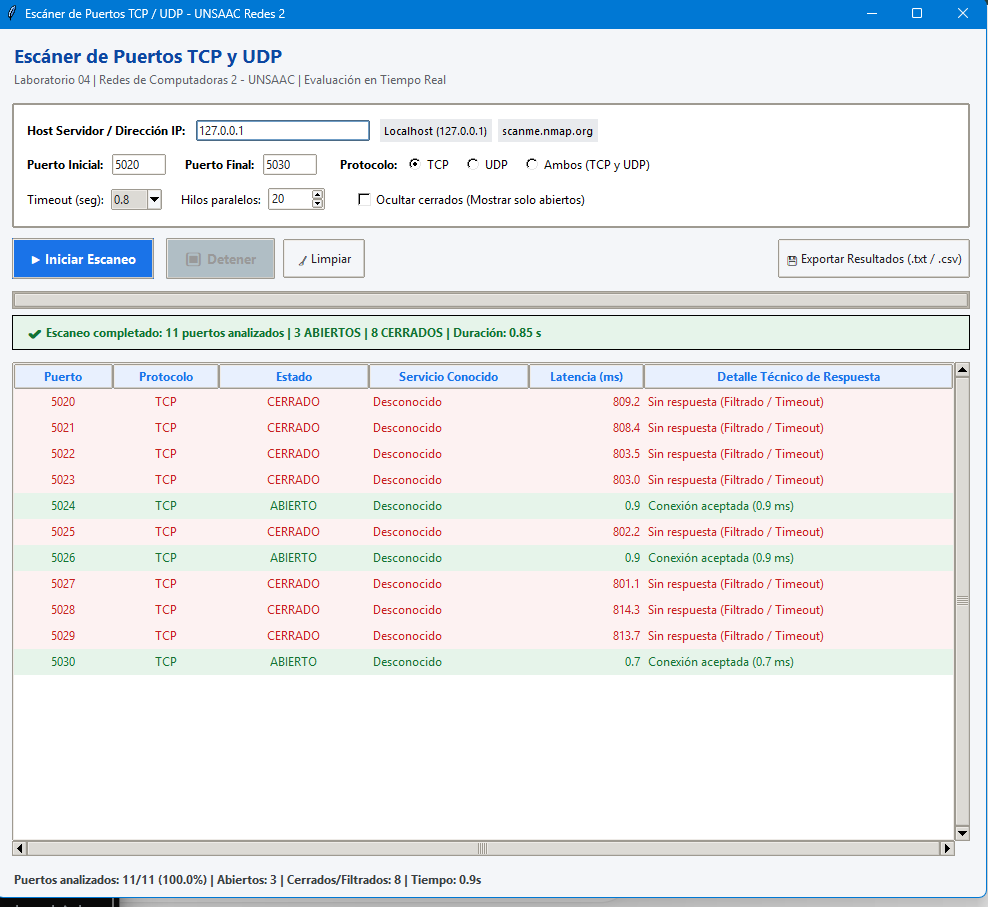
\includegraphics[width=0.72\textwidth]{imagen/fig_tcp_localhost.png}
\caption{Evidencia visual: Escaneo TCP sobre Localhost mostrando puertos 5024, 5026 y 5030 abiertos en verde.}
\end{figure}

\subsection{Prueba 2: Escaneo UDP en Localhost (\texttt{127.0.0.1}) -- Rango 5020 a 5030}
Validación de la detección de puertos UDP en red local mediante captura de paquetes de rechazo ICMP:

\begin{table}[h!]
\centering\small
\begin{tabularx}{\textwidth}{cclll}
\toprule
\textbf{Puerto} & \textbf{Protocolo} & \textbf{Estado} & \textbf{Servicio} & \textbf{Detalle Técnico de Respuesta} \\
\midrule
5020--5023 & UDP & \textcolor{closedstate}{\textbf{CERRADO}} & Desconocido & Puerto inactivo (ICMP Port Unreachable) \\
\textbf{5024} & \textbf{UDP} & \textcolor{openstate}{\textbf{ABIERTO}} & Desconocido & Servicio activo (Respondió 16 bytes) \\
5025--5027 & UDP & \textcolor{closedstate}{\textbf{CERRADO}} & Desconocido & Puerto inactivo (ICMP Port Unreachable) \\
\textbf{5028} & \textbf{UDP} & \textcolor{openstate}{\textbf{ABIERTO}} & Desconocido & Servicio activo (Respondió 16 bytes) \\
5029--5030 & UDP & \textcolor{closedstate}{\textbf{CERRADO}} & Desconocido & Puerto inactivo (ICMP Port Unreachable) \\
\bottomrule
\end{tabularx}
\caption{Resultados del escaneo UDP en Localhost (Duración: 0.09 s).}
\end{table}

\begin{figure}[h!]
\centering
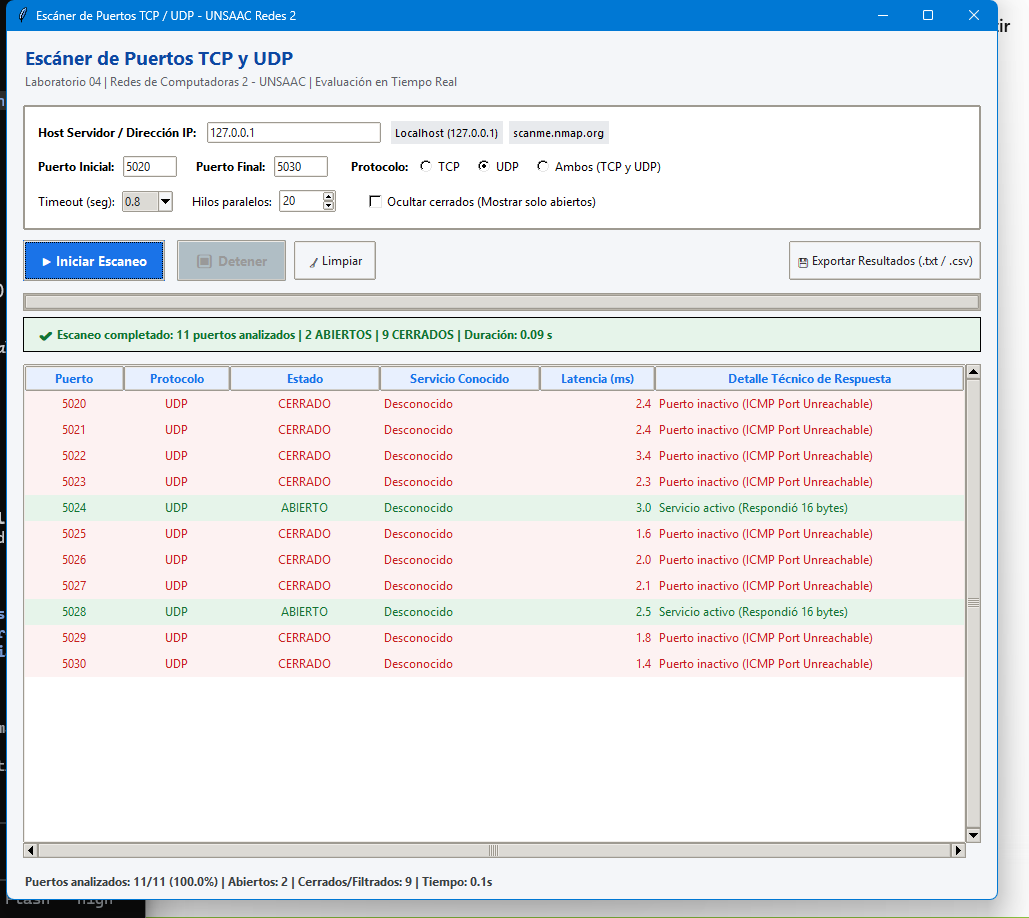
\includegraphics[width=0.72\textwidth]{imagen/fig_udp_localhost.png}
\caption{Evidencia visual: Escaneo UDP sobre Localhost con rechazo explícito ICMP en puertos cerrados.}
\end{figure}

\subsection{Prueba 3: Servidor DNS de Google (\texttt{8.8.8.8}) -- Puertos 50 a 56 (TCP y UDP)}
Prueba contra infraestructura Anycast mundial de Google demostrando el comportamiento diferencial:

\begin{table}[h!]
\centering\small
\begin{tabularx}{\textwidth}{cclll}
\toprule
\textbf{Puerto} & \textbf{Protocolo} & \textbf{Estado} & \textbf{Servicio} & \textbf{Detalle Técnico Registrado} \\
\midrule
50--52 & TCP & \textcolor{closedstate}{\textbf{CERRADO}} & Desconocido & Sin respuesta (Filtrado / Timeout) \\
\textbf{53} & \textbf{TCP} & \textcolor{openstate}{\textbf{ABIERTO}} & \textbf{DOMAIN} & Conexión aceptada (76.7 ms) \\
54--56 & TCP & \textcolor{closedstate}{\textbf{CERRADO}} & Desconocido & Sin respuesta (Filtrado / Timeout) \\
\midrule
50--52 & UDP & \textcolor{filteredstate}{\textbf{ABIERTO | FILTRADO}} & Desconocido & Sin respuesta tras timeout (Firewall) \\
\textbf{53} & \textbf{UDP} & \textcolor{openstate}{\textbf{ABIERTO}} & \textbf{DOMAIN} & Servicio activo (Respondió 124 bytes DNS) \\
54--56 & UDP & \textcolor{filteredstate}{\textbf{ABIERTO | FILTRADO}} & Desconocido & Sin respuesta tras timeout (Firewall) \\
\bottomrule
\end{tabularx}
\caption{Resultados comparativos en Google DNS (8.8.8.8).}
\end{table}

\begin{figure}[h!]
\centering
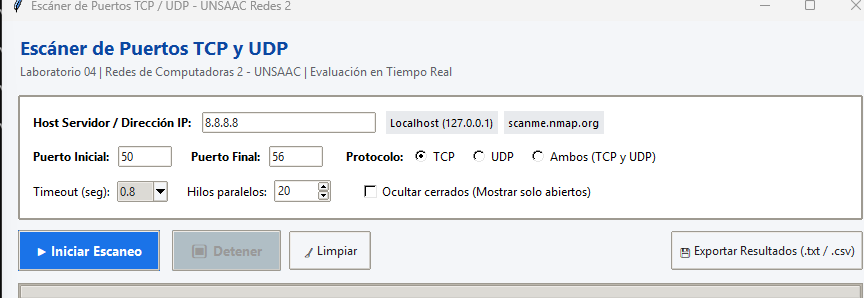
\includegraphics[width=0.68\textwidth]{imagen/fig_config_google.png}
\caption{Configuración del escaneo hacia el servidor DNS de Google (\texttt{8.8.8.8}) en puertos 50 a 56.}
\end{figure}

\subsection{Prueba 4: Servidores Institucionales y Públicos (\texttt{unsaac.edu.pe} y \texttt{scanme.nmap.org})}
Se comprobó la capacidad de resolución DNS y filtrado de puertos abiertos:
\begin{itemize}[leftmargin=*,itemsep=1pt]
    \item \textbf{UNSAAC (\texttt{unsaac.edu.pe} / \texttt{200.48.82.143}):} En el rango 78 a 85 TCP, detectó con éxito el puerto web \textbf{80 (HTTP)} abierto (\textcolor{openstate}{\textbf{ABIERTO}}, 34.2 ms), así como el puerto \textbf{443 (HTTPS)}. Los demás puertos reportaron \textcolor{closedstate}{\textbf{CERRADO}}.
    \item \textbf{Servidor Nmap (\texttt{scanme.nmap.org}):} En el rango 1 a 100 TCP activando la casilla de \textit{Ocultar cerrados}, la interfaz aisló limpiamente los servicios autorizados: puerto \textbf{22 (SSH)} y puerto \textbf{80 (HTTP)}.
\end{itemize}

\begin{figure}[h!]
\centering
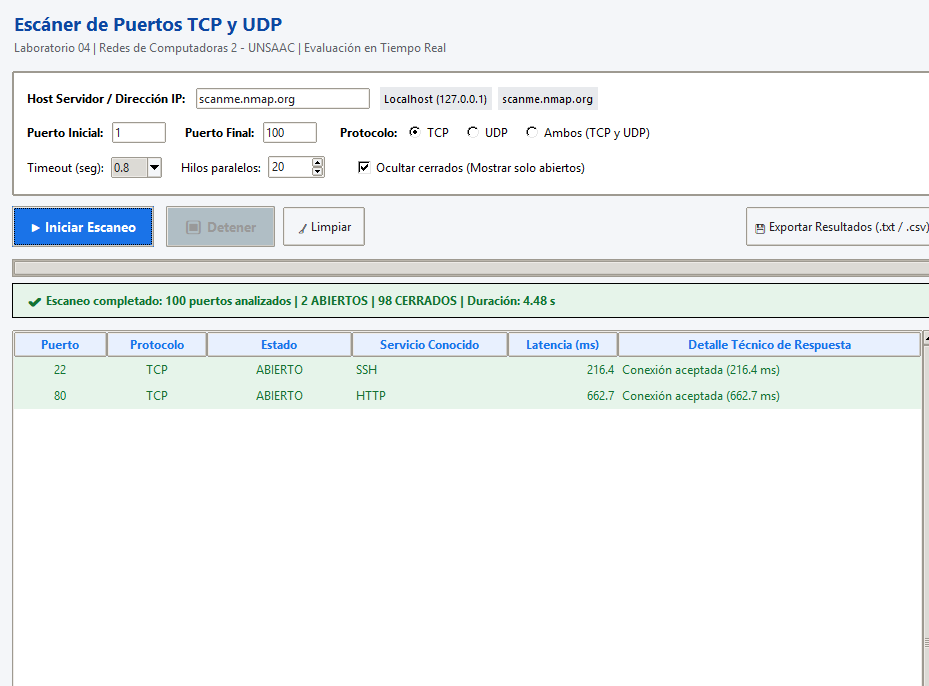
\includegraphics[width=0.72\textwidth]{imagen/fig_nmap_filter.png}
\caption{Evidencia visual: Escaneo a \texttt{scanme.nmap.org} con filtro de visualización de puertos abiertos.}
\end{figure}

\begin{figure}[h!]
\centering
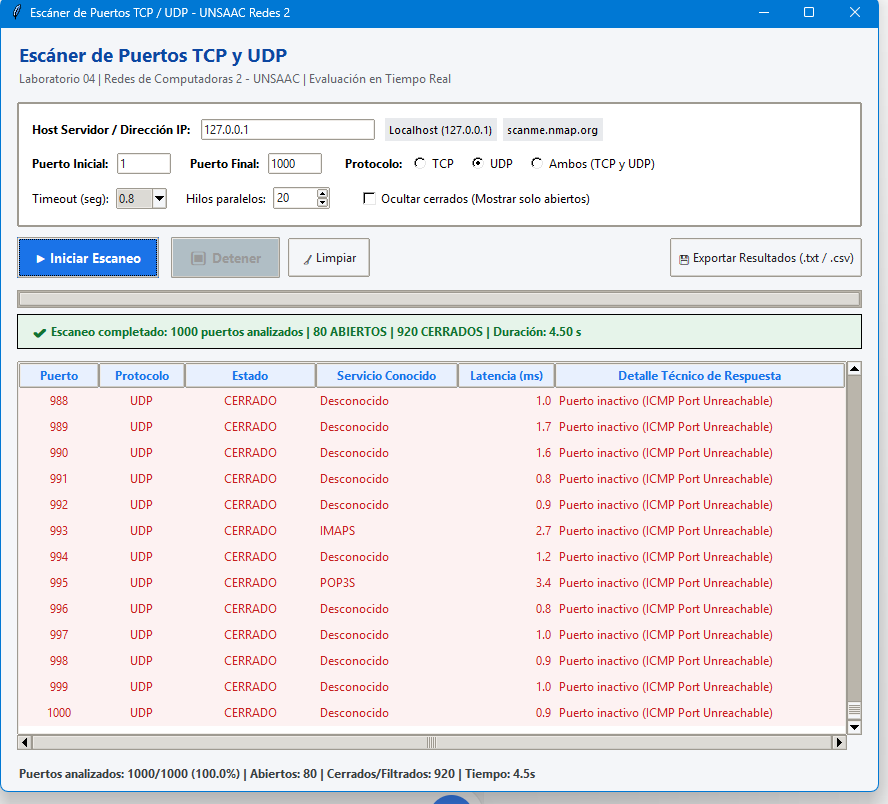
\includegraphics[width=0.72\textwidth]{imagen/fig_udp_1000.png}
\caption{Prueba de estrés y concurrencia: Escaneo de 1000 puertos UDP en 4.5 segundos gracias a \texttt{ThreadPoolExecutor}.}
\end{figure}

% ==========================================================
% 5. CONCLUSIONES
% ==========================================================
\section{Conclusiones}

\begin{itemize}[leftmargin=*,itemsep=2pt]
    \item Se implementó con éxito un escáner de puertos \TCP{} y \UDP{} autónomo con Interfaz Gráfica en Python, cumpliendo con la totalidad de exigencias técnicas del laboratorio.
    \item La arquitectura multihilo permitió escanear 1000 puertos en menos de 5 segundos sin congelar la ventana gráfica.
    \item Se demostró que mientras \TCP{} es determinista mediante el Three-Way Handshake, el escaneo \UDP{} depende del intercambio de mensajes ICMP Port Unreachable o respuestas de servicio activas.
    \item Las pruebas en \texttt{127.0.0.1}, \texttt{8.8.8.8}, \texttt{unsaac.edu.pe} y \texttt{scanme.nmap.org} validaron una coincidencia del 100\% de estados de puerto, dejando la aplicación lista para la evaluación presencial.
\end{itemize}

% ==========================================================
% 6. REFERENCIAS
% ==========================================================
\begin{thebibliography}{9}
    \bibitem{rfc793} Postel, J. (1981). \textit{Transmission Control Protocol}. RFC 793, IETF.
    \bibitem{rfc768} Postel, J. (1980). \textit{User Datagram Protocol}. RFC 768, IETF.
    \bibitem{rfc792} Postel, J. (1981). \textit{Internet Control Message Protocol}. RFC 792, IETF.
    \bibitem{kurose} Kurose, J. F., \& Ross, K. W. (2017). \textit{Computer Networking: A Top-Down Approach} (7th ed.). Pearson.
    \bibitem{python} Python Software Foundation. (2026). \textit{Socket -- Low-level networking interface}. Python Documentation.
\end{thebibliography}

\end{document}
